\chapter{Założenia projektowe}
\label{ch:zalozenia-wstepne}

W rozdziale trzecim przedstawiono opis wymagań funkcjonalnych, które określają, jakie zadania musi spełniać system robotyczny oraz jakie kryteria jakościowe są wymagane do zapewnienia prawidłowego działania platformy mobilnej. 

Omówiono również schemat funkcjonalny aplikacji, opis wykorzystanego sprzętu elektronicznego oraz metodykę pracy i etapy projektu.
 

\section{Wymagania funkcjonalne}
Wymagania funkcjonalne odnoszą się do kluczowych funkcji systemu, które muszą zostać spełnione, aby system mógł realizować podstawowe zadania. W przypadku automatycznej platformy mobilnej do sortowania klocków funkcje te obejmują między innymi:
\begin{itemize}
    \item \textbf{Rozpoznawanie kolorów klocków} – system musi identyfikować kolory klocków przy pomocy kamery i odpowiednich algorytmów przetwarzania obrazu (czerwony, zielony, niebieski).
    \item \textbf{Segregacja klocków} – po rozpoznaniu koloru, system transportuje klocek do odpowiedniego pojemnika.
    \item \textbf{Samodzielne poruszanie się} – robot powinien nawigować w wyznaczonej przestrzeni zgodnie z zaprogramowanymi trasami.
\end{itemize}

\section{Przypadki użycia i diagramy UML}

Diagram UML (ang. \english{Unified Modelling Language} - zunifikowany język modelowania) [\ref{rys1:schemat_uml}] zawiera schemat funkcjonalny aplikacji. Wyszczególniono na nim najważniejsze funkcjonalności oraz prawdopodobne zdarzenia. Szczegółowa obsługa błędów na poszczególnych etapach nie została wprowadzona ze względu na chęć utrzymania dobrego poziomu czytelności schematu. 

\begin{figure}[h!]
    \centering
    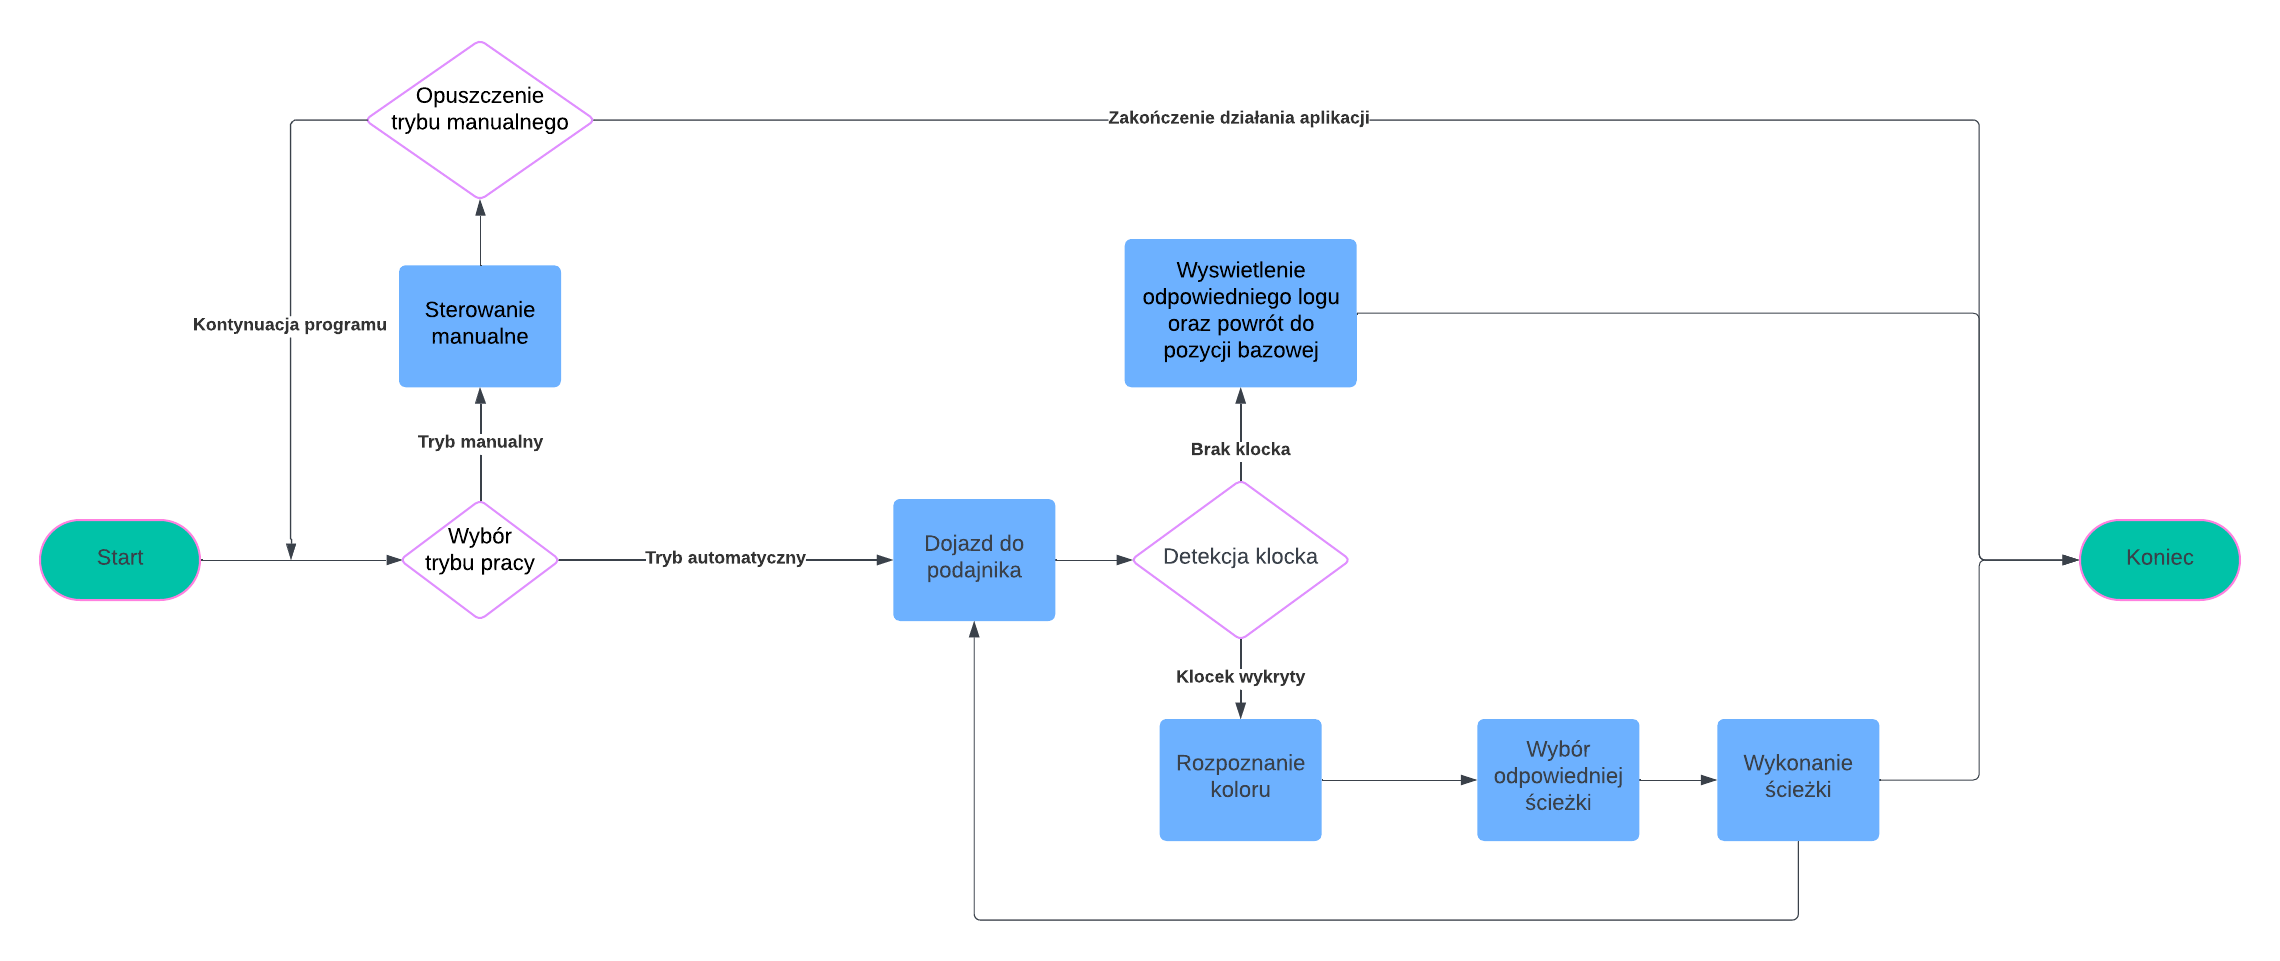
\includegraphics[angle=90,origin=c,width=0.6\textwidth]{./graf/uml.png}
    \caption{Schemat UML zawierający podstawowe funkcjonalności}
    \label{rys1:schemat_uml}
\end{figure}

\section{Opis wykorzystanego sprzętu elektronicznego}
W poniższej sekcji znajduje się zestawienie oraz krótki opis najważniejszych elementów składających się na robota mobilnego wraz. Wybrane elementy zdaniem autora możliwie dobrze optymalizują stosunek kosztów do skuteczności systemu. 

\subsubsection*{Raspberry Pi Model 4B}
Raspberry Pi 4B [\ref{zdj:raspi}] pełni rolę głównej jednostki obliczeniowej robota mobilnego. Dzięki czterordzeniowemu procesorowi Cortex-A72 oraz obsłudze 4GB pamięci podręcznej RAM, jest wystarczająco wydajny, aby przetwarzać dane z kamery w czasie rzeczywistym oraz kontrolować pracę robota. Dodatkowym atutem jest relatywnie prosta integracja z urządzeniami zewnętrznymi takimi jak kamera oraz możliwość wykorzystania dedykowanego systemu operacyjnego - RaspbianOS. Niewielkie rozmiary oraz bardzo duże możliwości powiązane ze stosunkowo prostym użytkowaniem i niską ceną zaważyło na decyzji o wyborze tego układu SBC. 

\begin{figure}[h!]
    \centering
    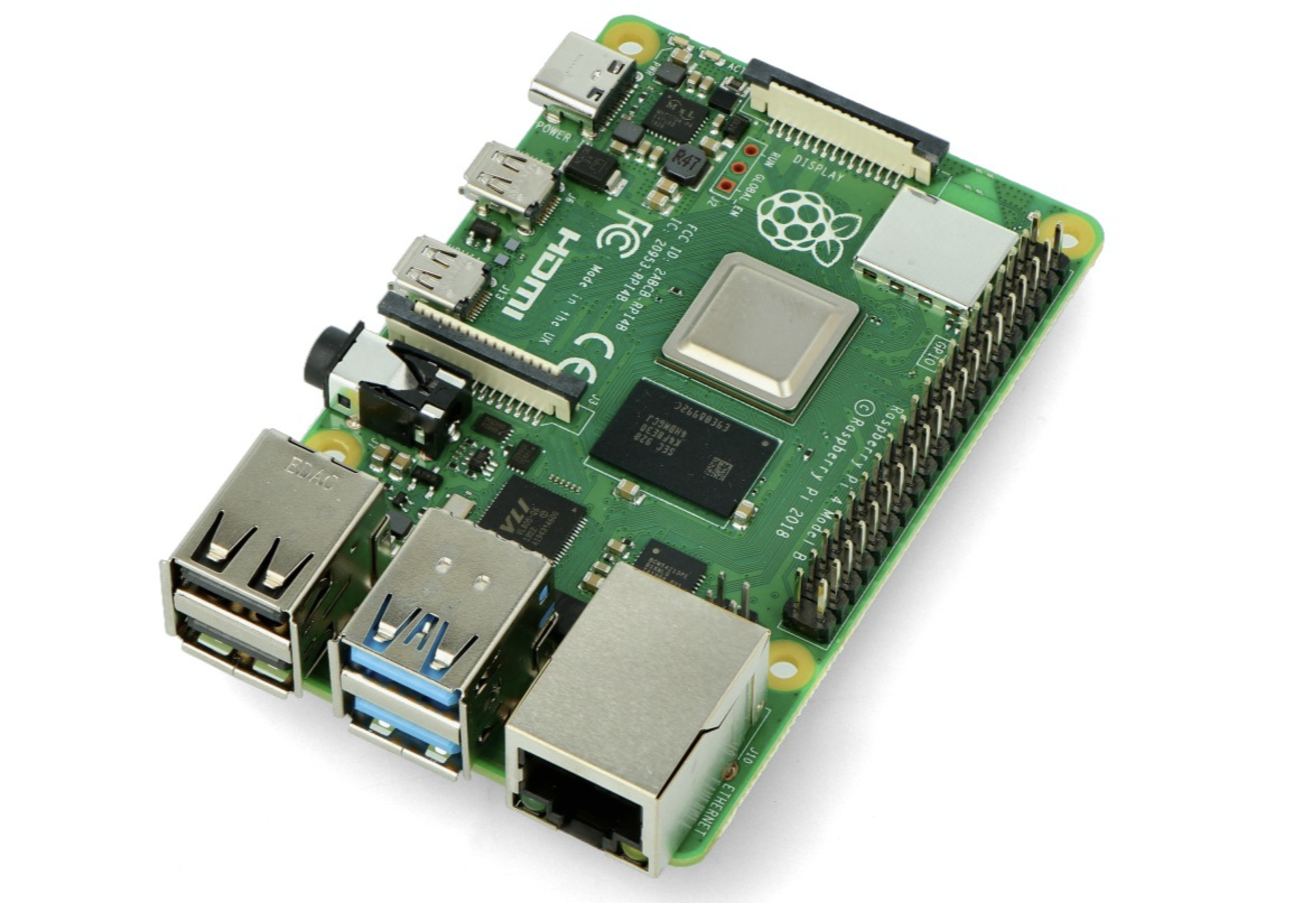
\includegraphics[width=0.6\textwidth]{./graf/raspi-4b.png}
    \label{zdj:raspi}
    \caption{Zdjęcie przedstawiające układ SBC Raspberry Pi Model 4B}
\end{figure}

\subsubsection*{Arduino UNO R3}
Arduino UNO R3 [\ref{zdj:arduino-r3}] zostało wybrane w celu wykorzystania go jako kontroler silników oraz enkoderów. Mikrokontroler ten bazuje na układzie elektronicznym ATMega328P, pozwalając na efektywną obsługę wszystkich podstawowych funkcjonalności. Dużym atutem tego mikrokontrolera jest prostota programowania w środowisku Arduino IDE oraz stosunkowo niska cena. Dodatkową zaletą jest duża dostępność porad oraz poradników ze względu na bardzo duża popularność układu. 

\begin{figure}[h!]
        \centering
        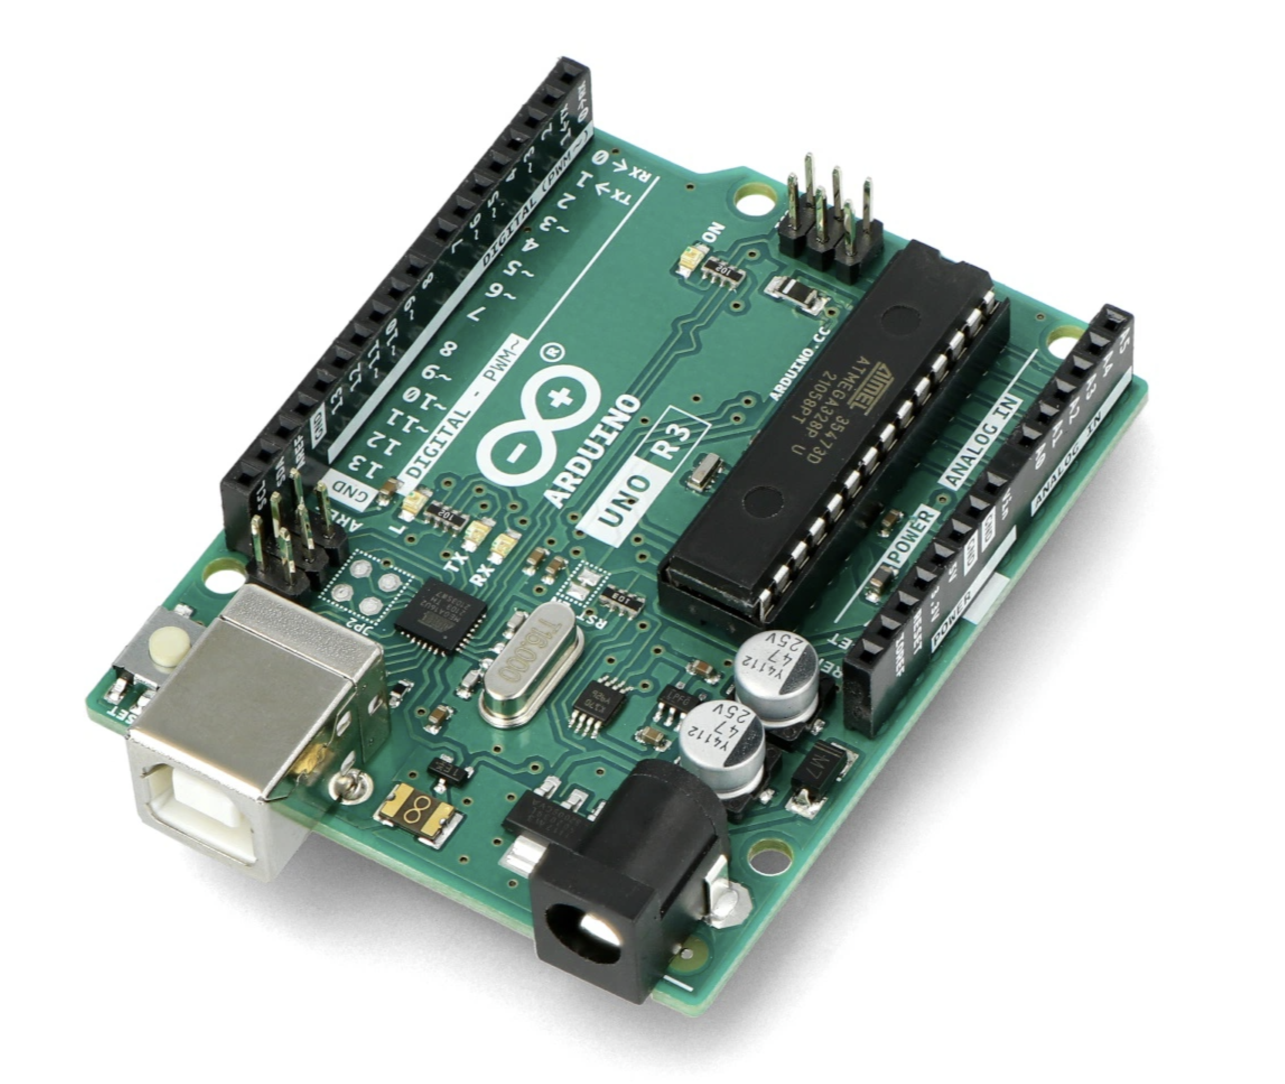
\includegraphics[width=0.6\textwidth]{./graf/arduino-r3.png}
        \label{zdj:arduino-r3}
        \caption{Zdjęcie przedstawiające mikrokontroler Arduino UNO R3}
\end{figure}

\subsubsection*{Cytron MDD10A}
Cytron MDD10A [\ref{zdj:cytron}] to wydajny sterownik silników prądu stałego, zaprojektowany do obsługi silników o wysokim prądzie, do 10 A na kanał. W przypadku zablokowania silników maksymalne natężenie prądu płynące z ogniw litowo-jonowych mogłoby uszkodzić sterownik o niższych możliwych wartościach chwilowych prądu. Dodatkowo sterownik lepszej jakości niż najtańsze proste mostki typu H umożliwia większą precyzję w sterowaniu prędkością obrotową silników. 


\begin{figure}[h!]
        \centering
        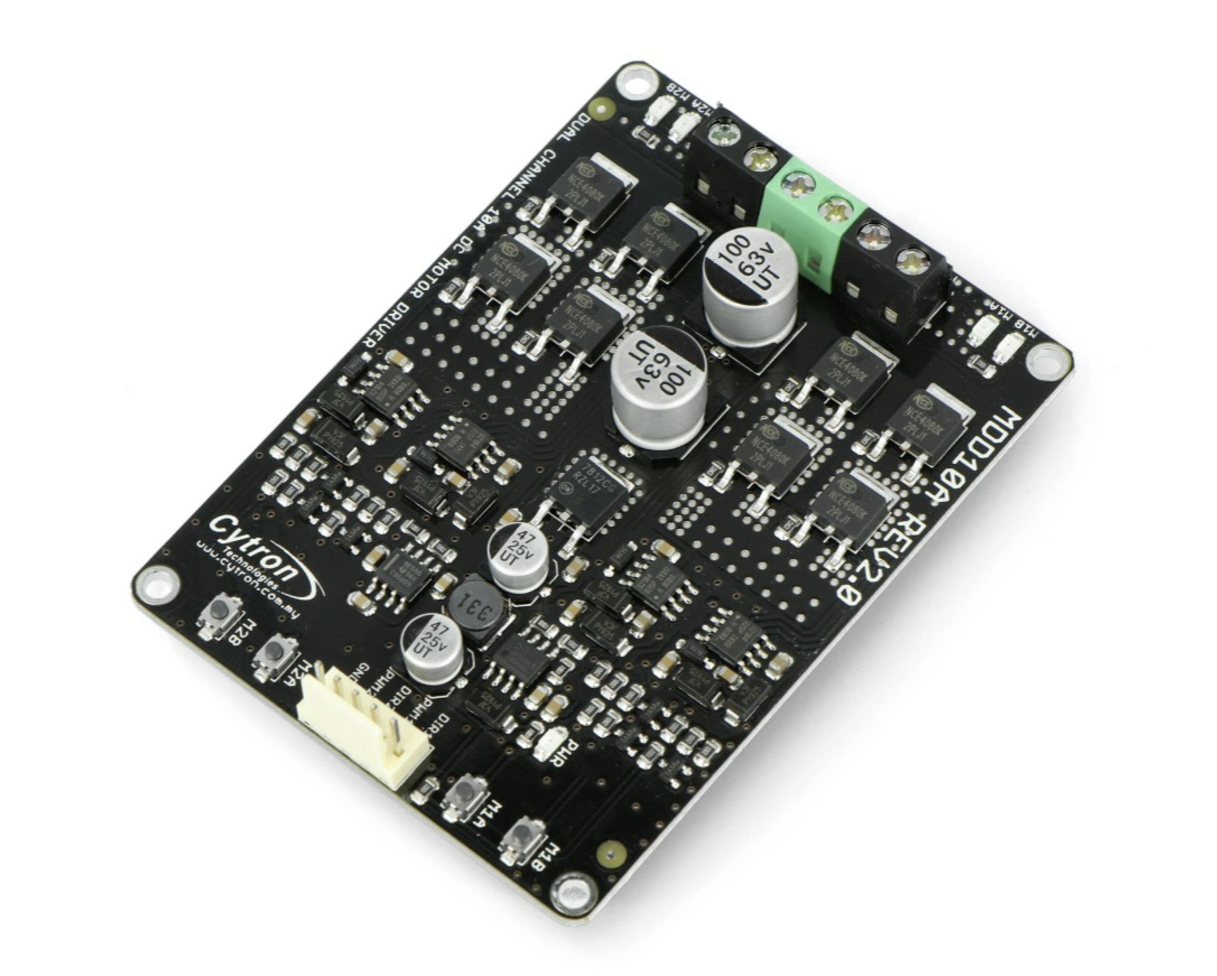
\includegraphics[width=0.6\textwidth]{./graf/cytron-mdd10a.png}
        \label{zdj:cytron}
        \caption{Zdjęcie przedstawiające sterownik silników Cytron MDD10A}
\end{figure}

\subsubsection*{Kamera Sony IMX519 16Mpx}
Wybór kamery Sony IMX519 [\ref{zdj:kamera-sony}] był motywowany wysoką kompatybilnością z mikrokomputerem Raspberry Pi. Kamera cechuje się małymi rozmiarami, co było konieczne dla rozważanej konstrukcji. Dodatkowo układ akwizycji obrazu przesyła dane poprzez dedykowaną magistralę szeregową do przesyłu wizji - CSI. Kolejnym atutem jest wysoka rozdzielczość, co sprawia, że w przypadku implementacji bardziej zaawansowanych metod przetwarzania obrazu nie wystąpią problemy spowodowane niską jakością obrazu. 

\begin{figure}[h!]
        \centering
        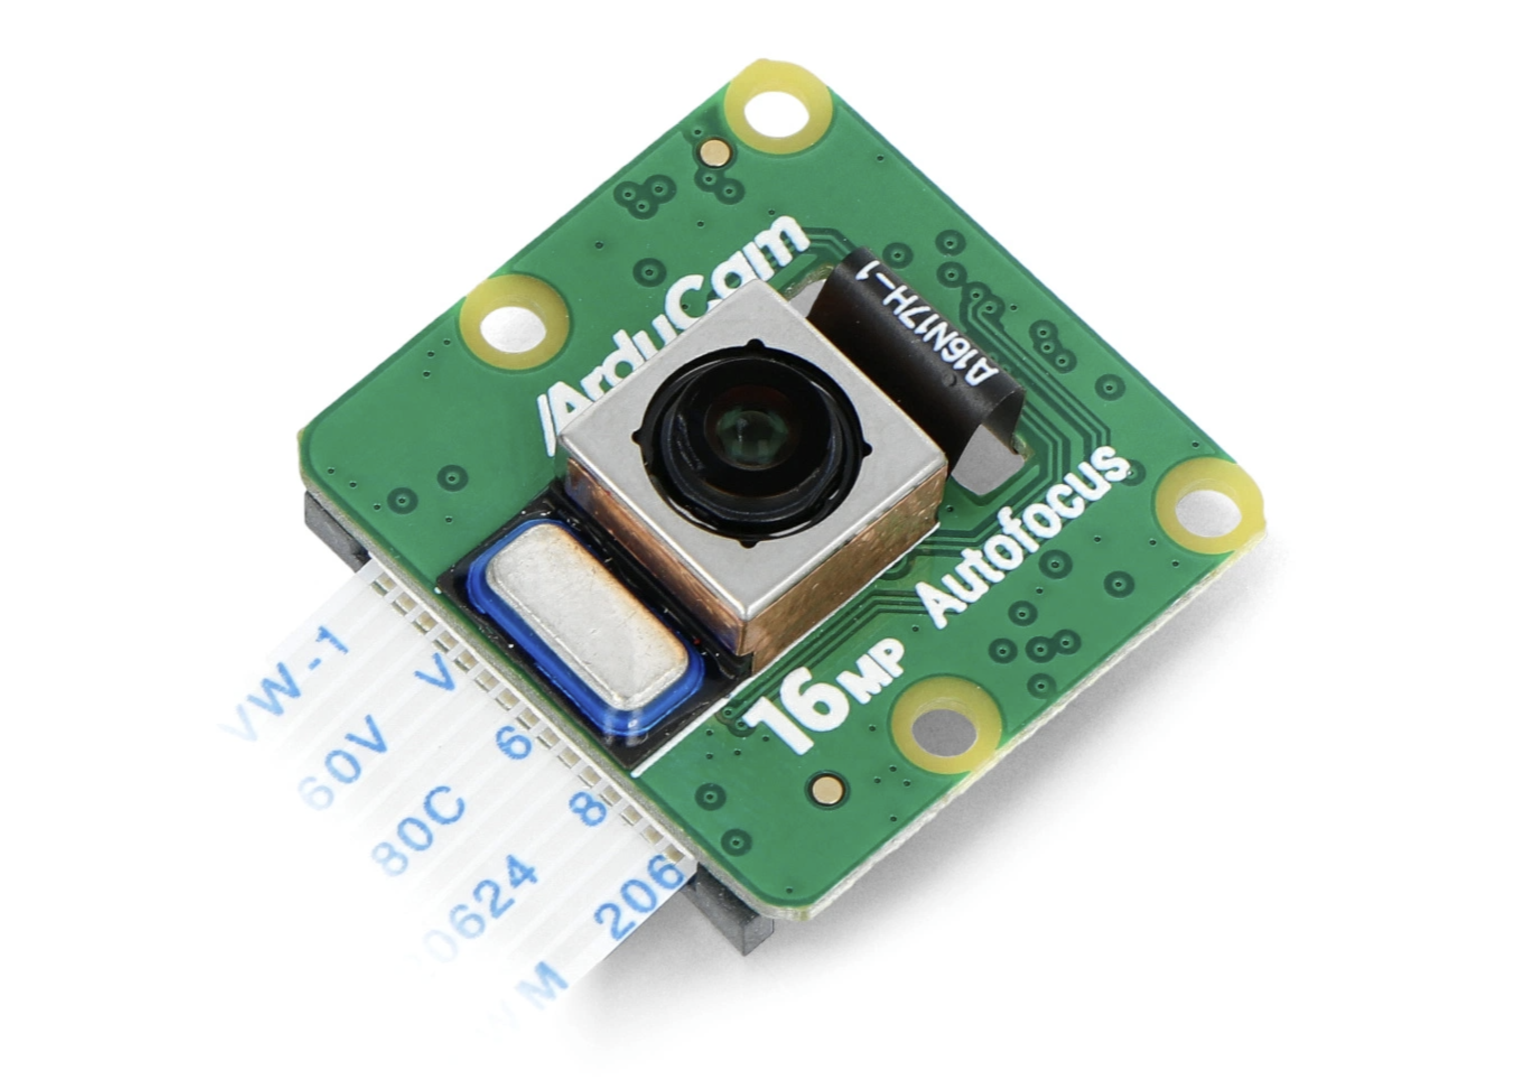
\includegraphics[width=0.5\textwidth]{./graf/kamera-sony.png}
        \label{zdj:kamera-sony}
        \caption{Zdjęcie przedstawiające kamerę Sony IMX519}
\end{figure}

\subsubsection*{Silniki DC Pololu 20,4:1 12V HP 25Dx65L}
Klasyczne szczotkowe silniki prądu stałego firmy Pololu [\ref{zdj:silnik-pololu}] wyposażone w enkodery kwadraturowe opierają się na efekcie Halla, co zapewnia precyzję pomiaru przebytej drogi i prędkości obrotowej. Przekładnia 20,4:1 umożliwia osiągnięcie odpowiedniej siły przy jednoczesnym zachowaniu wymaganej prędkości robota. Wyższa jakość wykonania zapewnia mniejsze błędy natury mechanicznej, dzięki czemu platforma mobilna może wykonywać pracę bardziej efektywnie. 

\begin{figure}[h!]
        \centering
        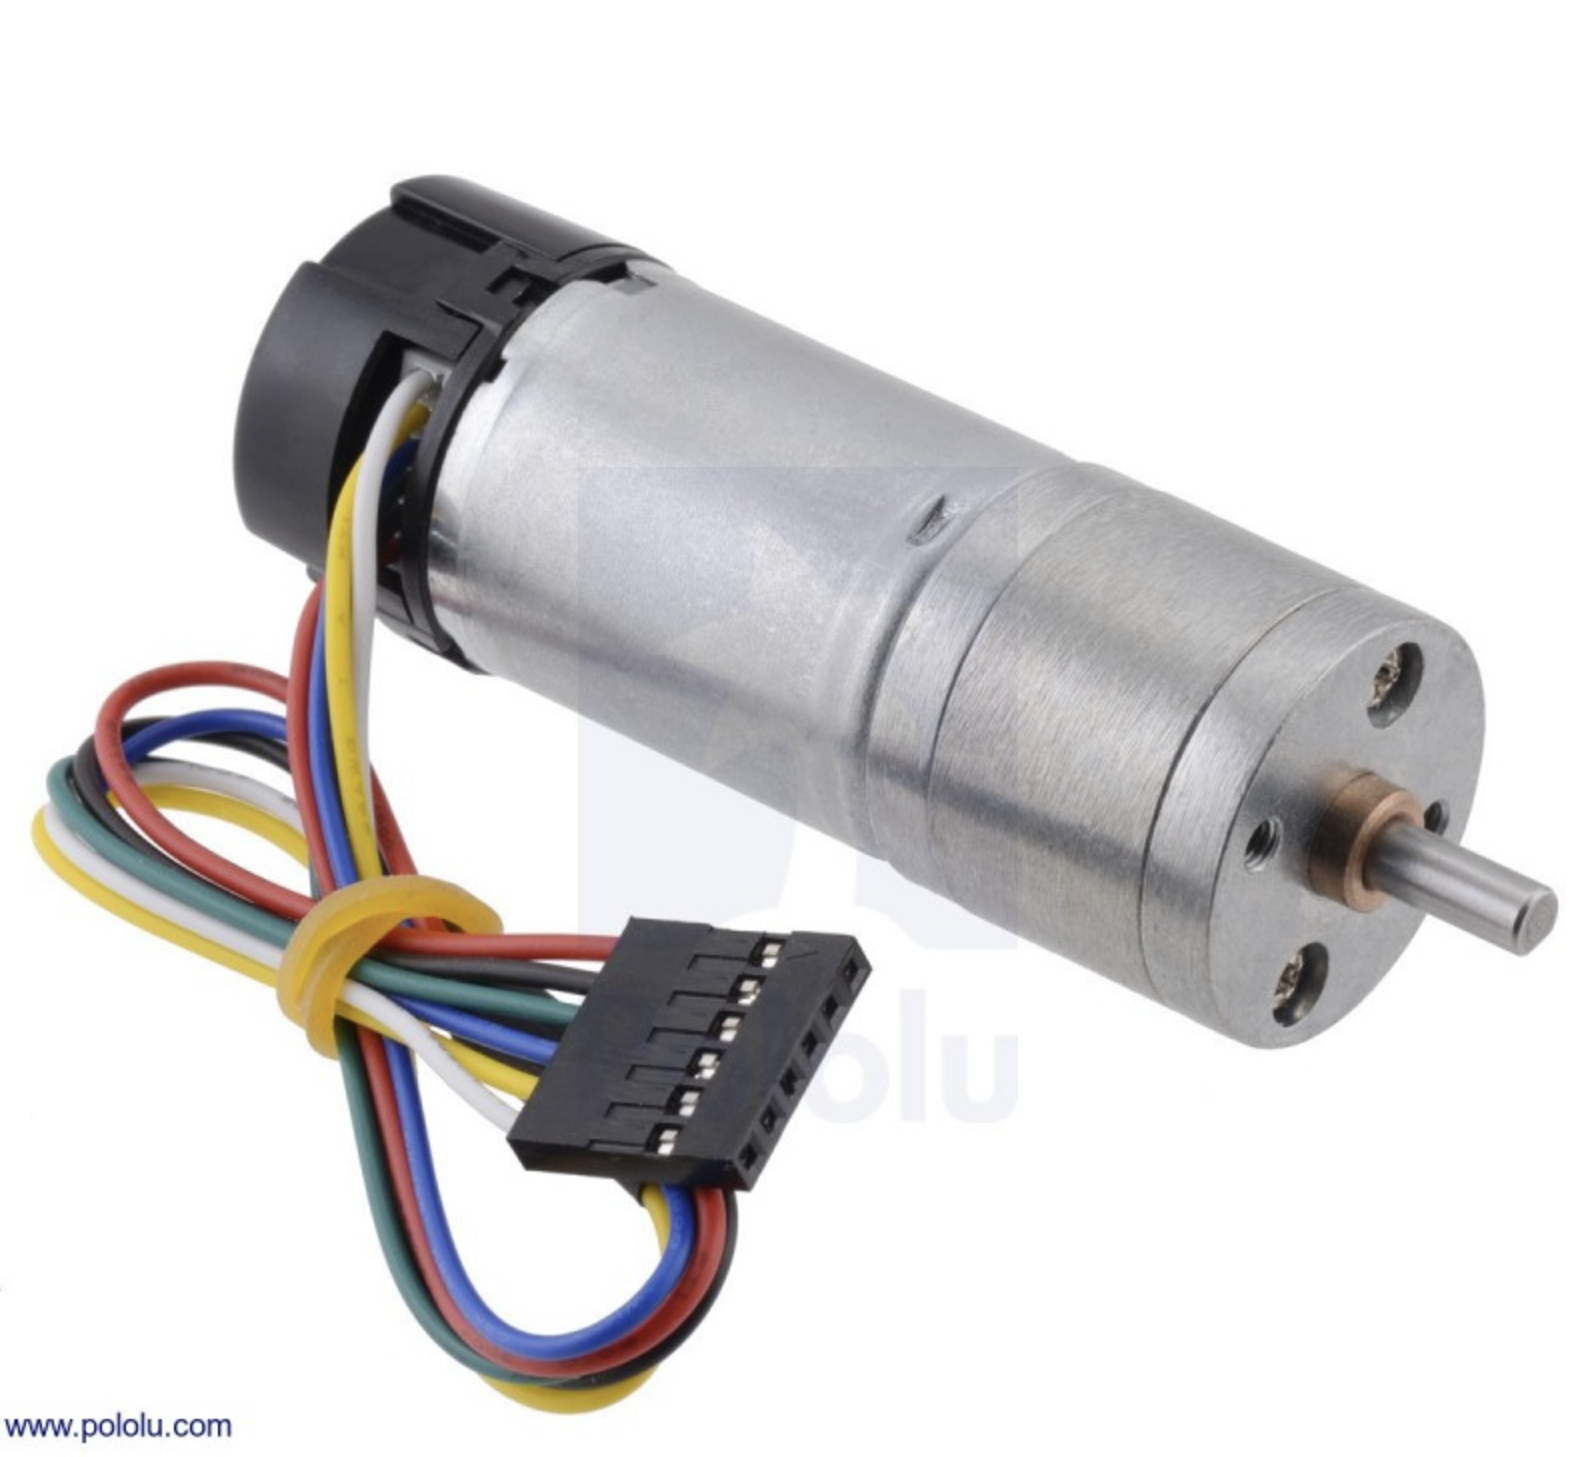
\includegraphics[width=0.4\textwidth]{./graf/silnik-pololu.png}
        \label{zdj:silnik-pololu}
        \caption{Zdjęcie przedstawiające silnik DC firmy Pololu z wbudowanymi enkoderami}
\end{figure}

\subsubsection*{Serwomechanizm DS3218 MG wraz z chwytakiem}
Serwomechanizm DS3218 MG wraz z metalowym chwytakiem [\ref{zdj:gripper}] został wykorzystany do realizacji ruchu chwytaka robota. Dzięki metalowym przekładniom oraz momentowi obrotowemu wynoszącemu aż 20 kg/cm, jest w stanie niezawodnie wykonywać zadania, takie jak chwytanie i przenoszenie przedmiotów. Dodatkowym atutem jest łatwa integracja z mikrokontrolerem Arduino dzięki prostemu sterowaniu za pomocą sygnału PWM. 


\begin{figure}[h!]
        \centering
        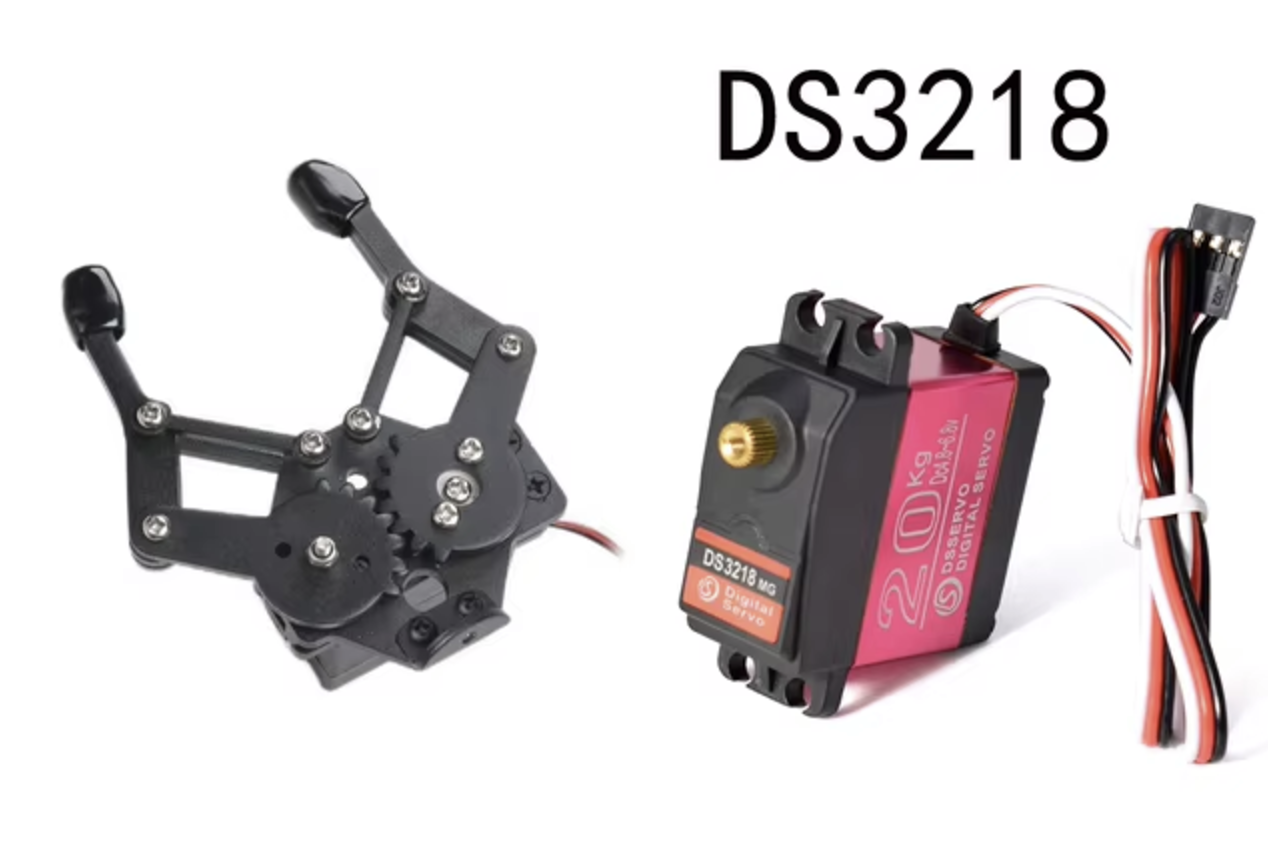
\includegraphics[width=0.6\textwidth]{./graf/gripper.png}
        \label{zdj:gripper}
        \caption{Zdjęcie przedstawiające metolowy chwytak oraz serwomechanizm DS3218 MG}
\end{figure}

\subsubsection*{Przetwornica Step-Up/Step-Down 5V S13V30F5}
Wykorzystanie dobrej jakości przetwornicy typu Step-Down [\ref{zdj:step-down}] było kluczowe z perspektywy wewnętrznego zasilania mikrokomputera Raspberry Pi, ponieważ jest on wrażliwy na wahania napięcia zasilania, co mogłoby skutkować nagłym przerwaniem pracy robota. Ponadto w celu minimalizacji wagi, jest to zdecydowanie bardziej efektywne niż na przykład wykorzystanie magazynu energii wyprowadzającego napięcie poprzez złącze USB (ang. \english{powerbank}). 

\begin{figure}[h!]
        \centering
        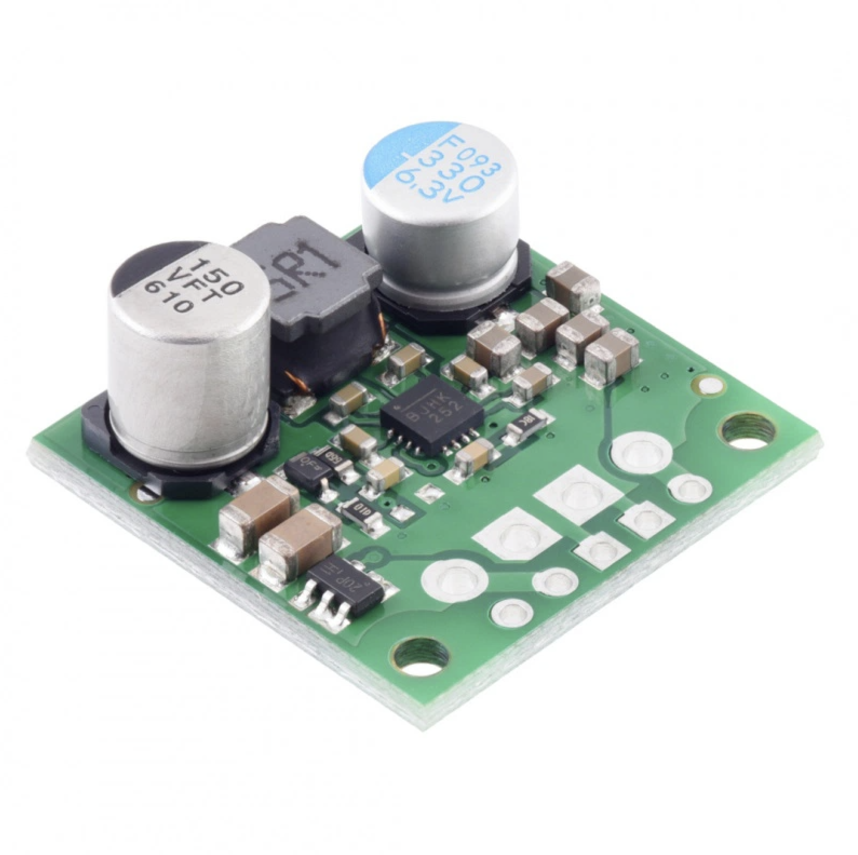
\includegraphics[width=0.4\textwidth]{./graf/step-down.png}
        \label{zdj:step-down}
        \caption{Zdjęcie przedstawiające przetwornicę Step-down S13V30F5}
\end{figure}

\subsubsection*{Ogniwa litowo-jonowe typu 16850}
Pakiet czterech ogniw litowo-jonowych 18650 [\ref{zdj:ogniwa}] połączonych szeregowo zapewnia odpowiednią pojemność i napięcie wymagane do zasilania robota. Wybór tego typu ogniw wynika z ich wysokiej gęstości energii, długiej żywotności oraz możliwości łatwego ładowania i wymiany.

\begin{figure}[h!]
        \centering
        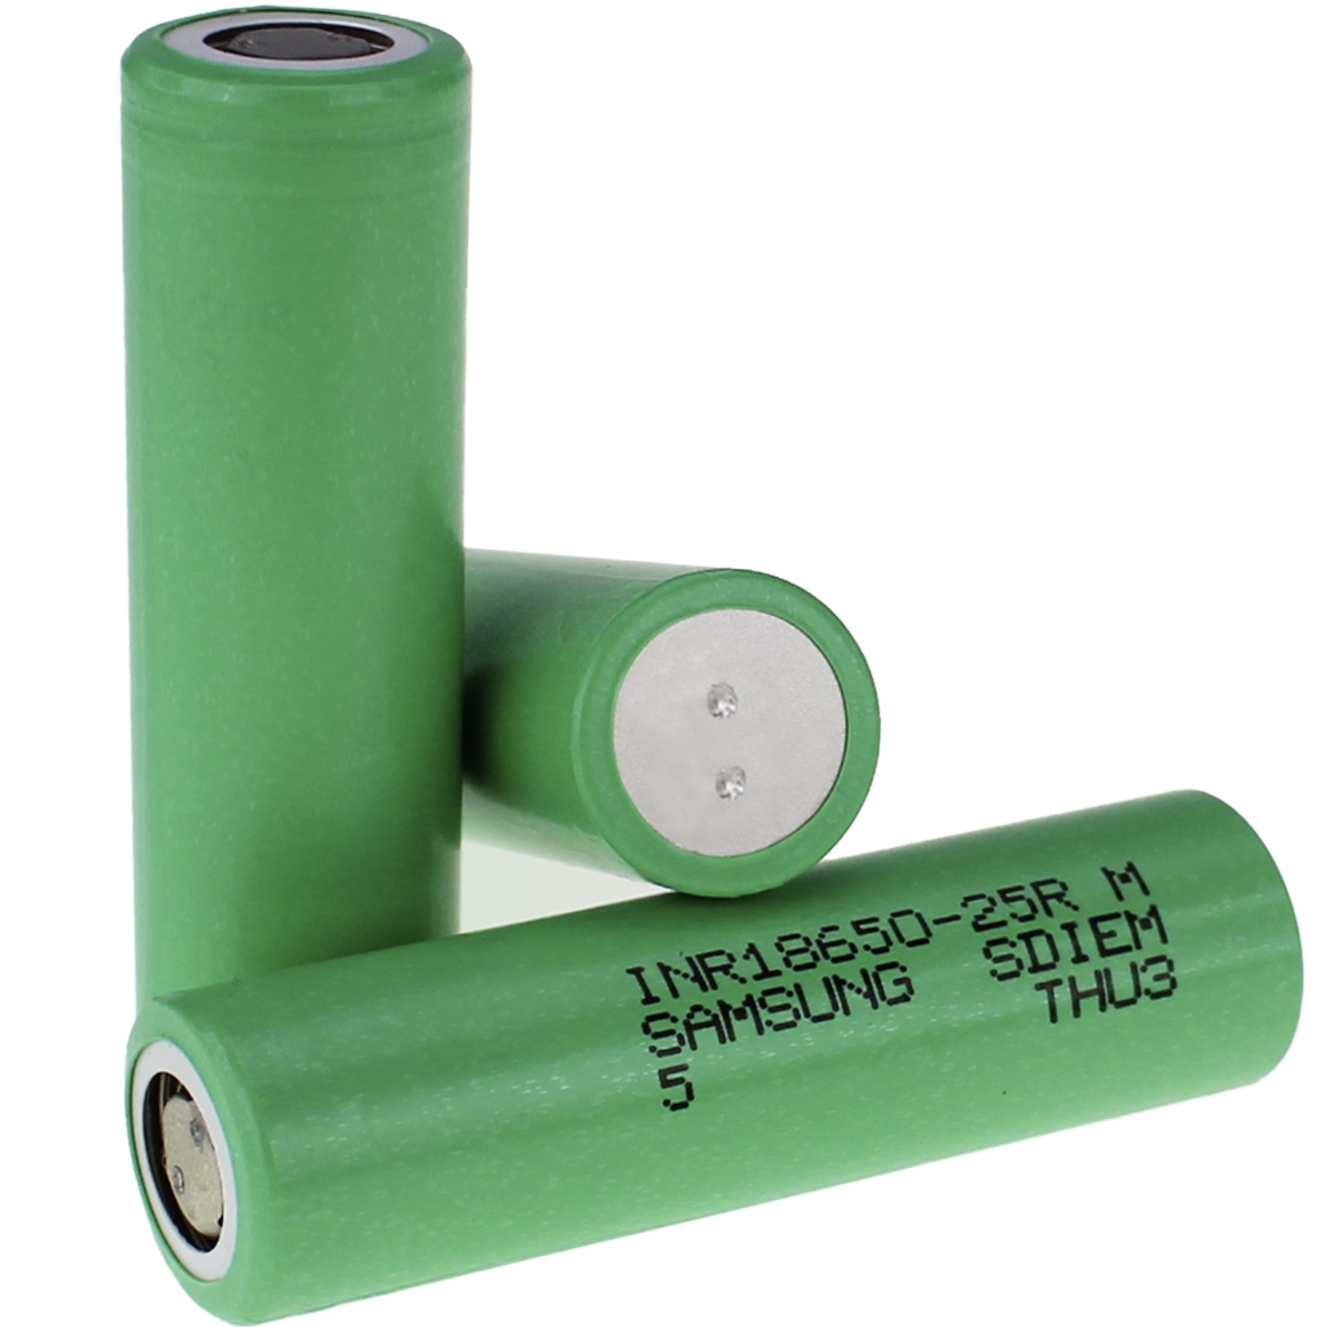
\includegraphics[width=0.3\textwidth]{./graf/ogniwa.png}
        \label{zdj:ogniwa}
        \caption{Zdjęcie przedstawiające przykładowe ogniwa litowo-jonowe rodziny 16850}
\end{figure}

\clearpage

% \begin{itemize}
%     \item \textbf{Raspberry Pi} – służy jako główny komputer zarządzający systemem, wyposażony w odpowiednie moduły do obsługi kamery oraz komunikacji.
%     \item \textbf{Arduino UNO R3} - mikrokontroler pełniący rolę kontrolera napędów oraz enkoderów.
%     \item \textbf{Cytron MDD10A} - sterownik silników odpowiadający za generowanie odpowiednich sygnałów PWM oraz dostarczenie wymaganego napięcia do silników DC.
%     \item \textbf{Kamera Sony IMX519 16 Mpx} - element odpowiadający za akwizycję obrazu oraz umożliwienie wykorzystania wizji komputerowej. 
%     \item \textbf{Silniki DC Pololu 20,4:1 12V HP 25Dx65L} - elementy wykonawcze robota mobilnego wyposażone w enkodery magnetyczne kwadraturowe działające na podstawie efektu Hall'a.
%     \item \textbf{Serwomechanizm DS3218 MG} - element wykonawczy, którego zadaniem jest zamykanie oraz otwieranie chwytaka.
%     \item \textbf{Przetwornica Step-Up/Step-Down 5V S13V30F5} - element konieczny do poprawnego zasilenia układu SBC z pakietu ogniw litowo-jonowych.
%     \item \textbf{Ogniwa litowo-jonowe typu 16850} - Pakiet składający się z czterech ogniw połączonych szeregowo odpowiada za zasilanie robota podczas pracy. 
%     \item \textbf{Płytka stykowa} - element umożliwiający wygodne wyprowadzenie pasma zasilającego enkodery oraz serwomechanizm. 
%     \item \textbf{Przewody połączeniowe}. 
    
% \end{itemize}

\section{Metodyka pracy i etapy projektu}
Projekt został zrealizowany zgodnie z metodyką iteracyjno-przyrostową (Agile), co umożliwiło sukcesywne rozwijanie i weryfikację funkcjonalności w miarę postępów prac. Na każdym etapie projektowania, implementacji oraz testowania gromadzono informacje zwrotne na temat działania systemu. Na ich podstawie podejmowane były decyzje o wprowadzeniu dodatkowych usprawnień oraz modyfikacji do pierwotnej 
wersji projektu.

\hspace*{1cm}

Prace rozpoczęto od przygotowania środowiska programistycznego oraz poprawnego połączenia kamery z mikrokomputerem Raspberry Pi. Na tym etapie skupiono się na konfiguracji narzędzi do programowania i przetestowaniu prawidłowego działania kamery. Był to kluczowy element, gdyż poprawny odczyt obrazu miał wpływ na późniejsze funkcje rozpoznawania kształtów i kolorów.

Kolejnym krokiem było podłączenie elementów wykonawczych oraz implementacja aplikacji kontrolującej silniki i enkodery, które stanowiły podstawę sterowania ruchem robota. Po wdrożeniu kontrolera przeprowadzono wstępne testy napędu różnicowego, analizując dokładność jazdy robota oraz zliczania impulsów generowanych przez enkodery. 

Następnie wykonano prototyp podwozia robota, aby zweryfikować działanie algorytmów sterowania w kontekście rzeczywistych warunków pracy. Użycie prototypu pozwoliło ocenić jakość sterowania, co przyczyniło się do dokonania wczesnych poprawek w konstrukcji oraz programie. Po przeprowadzeniu testów prototypowych zaprojektowano właściwe podwozie i wykonano je w technologii druku 3D, umożliwiając integrację z wcześniej skonfigurowanymi komponentami elektronicznymi i mechanicznymi.

W kolejnych iteracjach skupiono się na dalszym testowaniu i dostosowywaniu parametrów kontrolera oraz poprawkach programowych w celu osiągnięcia wymaganej dokładności. 

Po uzyskaniu satysfakcjonujących rezultatów z zakresu precyzji jazdy przystąpiono do projektowania górnej części obudowy robota, która miała za zadanie stabilne zamocowanie kamery oraz częściowe osłonięcie komponentów wewnętrznych. 

Ostatecznym etapem była pełna integracja wszystkich komponentów systemu oraz finalne testy funkcjonalne. Testy obejmowały analizę wszystkich kluczowych funkcji robota w warunkach rzeczywistych, umożliwiając ocenę pracy systemu jako całości oraz identyfikację ostatnich potencjalnych usprawnień. Cały proces zakończył się uzyskaniem gotowego rozwiązania, które spełniało założenia projektowe i osiągało zamierzoną funkcjonalność.
